\section{Azura}\label{azura}

Tags: Città, Sede Gilda Creatore: Davide, Lorenzo Ispirazione: Napoli
Luogo: Valtara

\section{Azura}\label{azura-1}

\begin{center}\rule{0.5\linewidth}{0.5pt}\end{center}

\begin{figure}
\centering
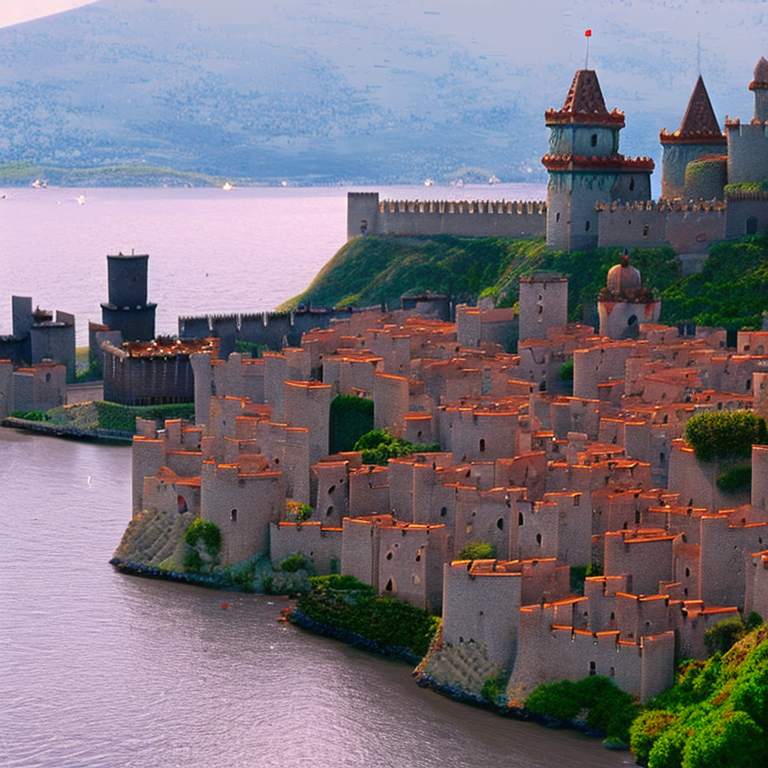
\includegraphics{a-large-medieval-city-by-the-see-it-has-a-port-walls-and-some-towers-.png}
\caption{a-large-medieval-city-by-the-see-it-has-a-port-walls-and-some-towers-.png}
\end{figure}

Informazioni Generali

Tipo di Luogo: Città-Stato

Dimensioni: 73.8 km²

Altitudine: 37 m s.l.m.

Popolazione: 122.267

Paese:

Luogo:

Alleata con:

Attività: Porto commerciale, Gilda dei protettori

\begin{center}\rule{0.5\linewidth}{0.5pt}\end{center}

\subsection{1. Descrizione Generale}\label{descrizione-generale}

\begin{center}\rule{0.5\linewidth}{0.5pt}\end{center}

\begin{figure}
\centering
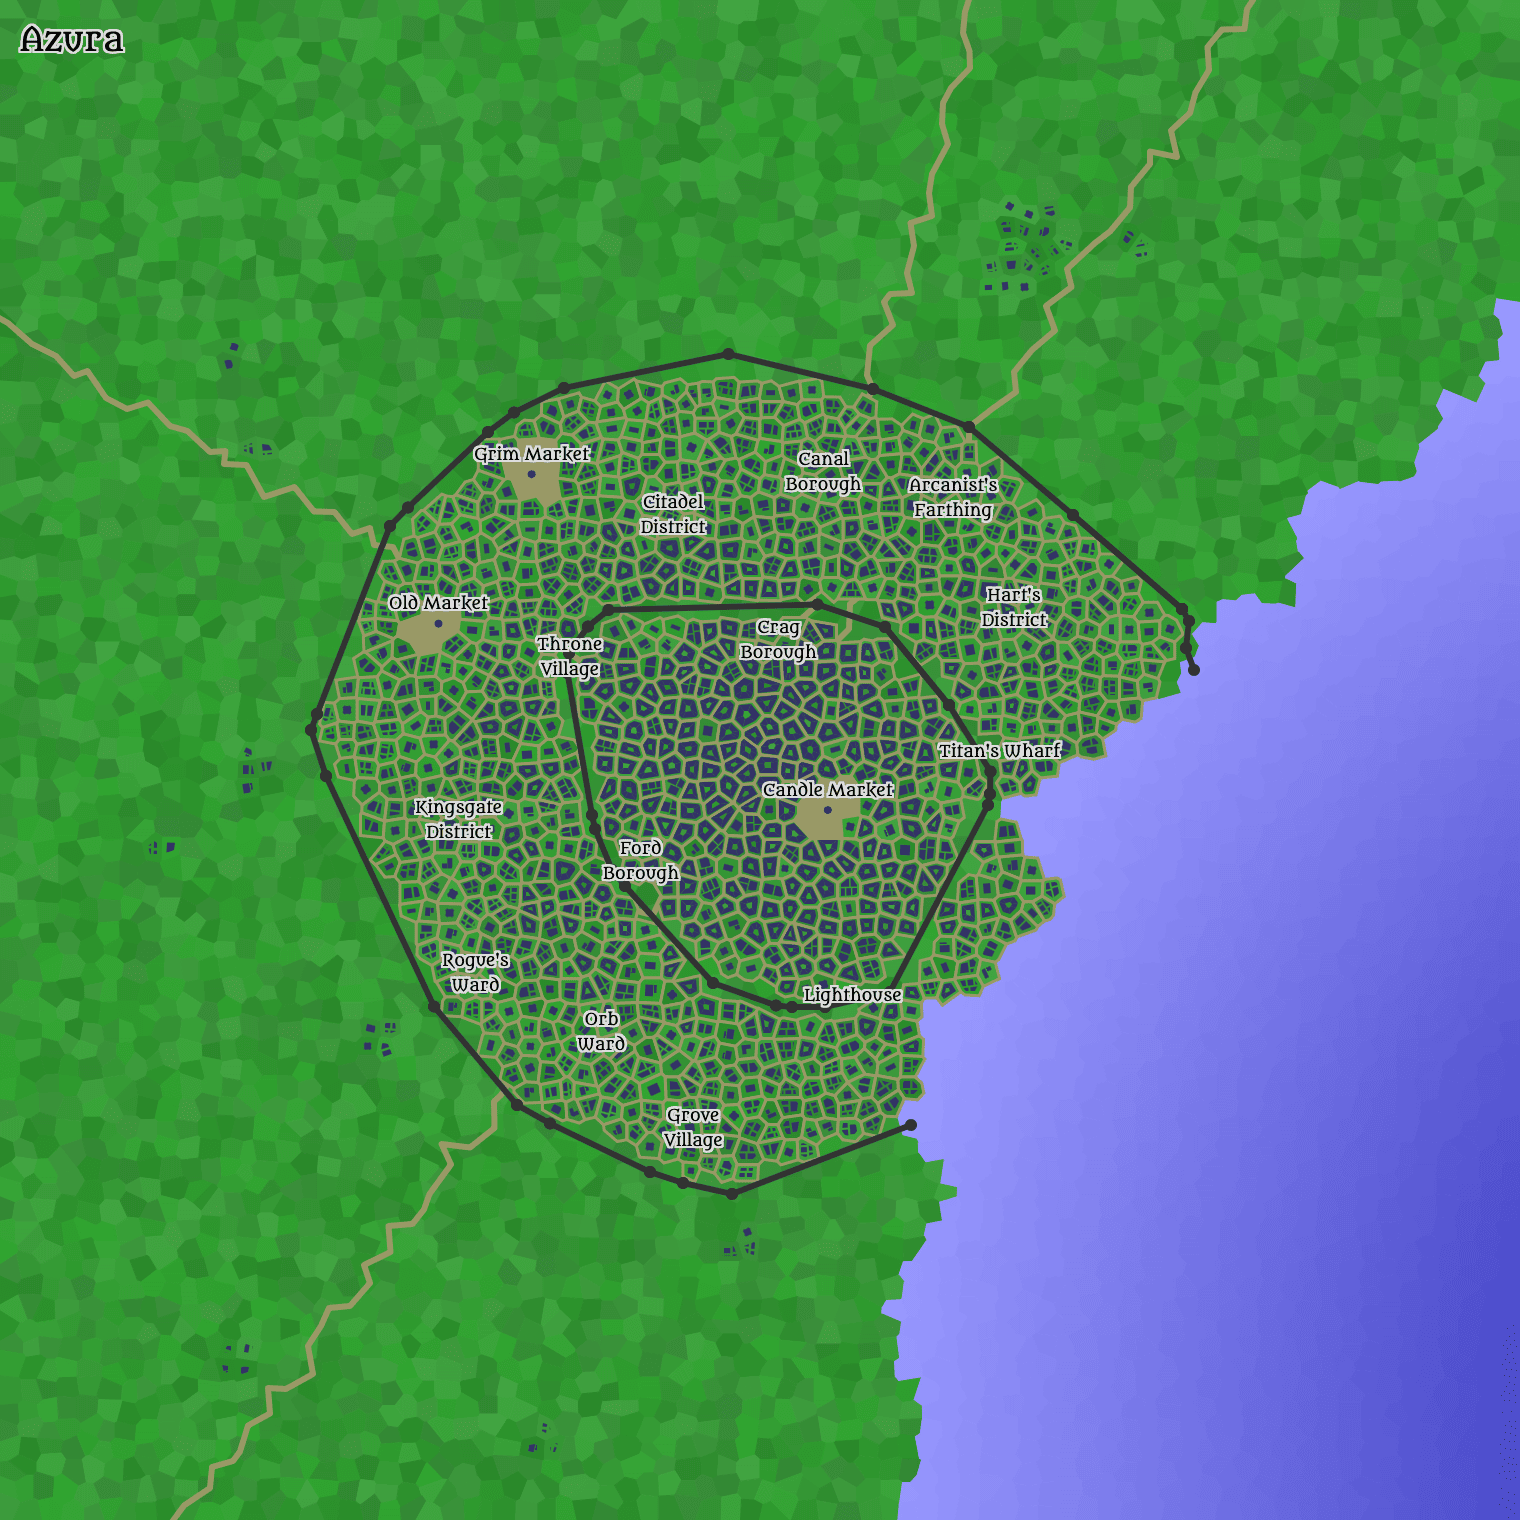
\includegraphics{Azura.png}
\caption{Azura.png}
\end{figure}

Azura è una città stato indipendente che sorge sulle coste del Mar di
Smeraldo, un luogo incantevole dalle acque cristalline che attraggono
visitatori da tutto il mondo. Tuttavia, dietro la facciata di città
splendente, si nascondono anche quartieri degradati e la corruzione. Non
tutti gli abitanti della città beneficiano della ricchezza e del potere
che Azura esercita sulle regioni circostanti. La città è governata da un
sistema politico fortemente centralizzato, che garantisce l'ordine
pubblico e la sicurezza, ma allo stesso tempo perpetua le disuguaglianze
sociali e la corruzione tra i ranghi più alti del potere. Gli abitanti
dei quartieri più poveri spesso vivono in condizioni precarie, senza
accesso ai servizi essenziali come l'acqua potabile e
l'elettricità.~Nonostante questi lati oscuri, Azura rimane una città
vivace e pulsante, con una scena culturale e artistica che attira
visitatori da tutto il mondo. La città è nota anche per la sua cucina,
che combina sapientemente tradizione e innovazione. Tuttavia, per i
personaggi che si addentrano nei suoi quartieri meno noti, Azura può
rivelarsi una città pericolosa e imprevedibile.

\begin{quote}
``Si Azura avvisa i montagne, fussa 'na piccola Kos'' - detto popolare
\end{quote}

\subsection{2. Storia}\label{storia}

\begin{center}\rule{0.5\linewidth}{0.5pt}\end{center}

La città di Azura fu fondata molti secoli fa da un gruppo di esploratori
che navigavano lungo la costa. La zona era ricca di risorse naturali e
la vicinanza con lo stretto offriva una naturale posizione strategica
per il commercio. Inizialmente la città era un piccolo villaggio di
pescatori, ma in poco tempo si sviluppò in un centro commerciale di
grande importanza, grazie alla sua posizione strategica e alle ricchezze
naturali della regione circostante. La città di Azura divenne ben presto
una città-stato indipendente, governata da un consiglio di mercanti e di
aristocratici. Negli anni successivi, Azura divenne famosa per la sua
bellezza, le sue architetture eleganti e le sue ricchezze. Tuttavia, non
tutto era dorato come sembrava. La corruzione, l'ingiustizia sociale e
la criminalità cominciarono ad insinuarsi all'interno della città, e
questa divenne un luogo dove l'opulenza e la povertà convivevano fianco
a fianco. Nonostante ciò, Azura è ancora una delle città più importanti
e ricche del Mar di Smeraldo, ma la sua bellezza è ora offuscata dalla
presenza di quartieri degradati e dalla corruzione. Secoli or sono la
città fu investita da una forte epidemia, che ne decimò la popolazione.
Da allora tutti i morti di Azura vengono cremati e degli antichi
cimiteri non c'è quasi più traccia.

\subsection{3. Geografia}\label{geografia}

\begin{center}\rule{0.5\linewidth}{0.5pt}\end{center}

\subsection{4. Demografia}\label{demografia}

\begin{center}\rule{0.5\linewidth}{0.5pt}\end{center}

Azura è una città relativamente grande, ma non eccessivamente affollata.
Circa 18.000 persone vivono all'interno dei suoi confini. La maggior
parte della popolazione è composta da umani ed elfi, ma ci sono anche
diverse minoranze rappresentate da altre razze, come nani e gnomi. La
città attrae molte persone in cerca di lavoro, sia da altre parti del
regno che da paesi stranieri, grazie alla sua reputazione di essere una
città prospera. Tuttavia, la città ha anche una quota significativa di
poveri e diseredati, soprattutto nelle zone più degradate e abbandonate
della città. La classe media e la classe alta si concentrano soprattutto
nelle zone più centrali della città.

\subsection{5. Economia}\label{economia}

\begin{center}\rule{0.5\linewidth}{0.5pt}\end{center}

Azura è una città molto attiva sul fronte commerciale, grazie alla sua
posizione strategica sul mare e alla sua prosperità economica. Ci sono
numerose attività commerciali in città, tra cui mercati all'aperto,
negozi di artigianato, taverne e locande, banchi di cambio, negozi di
stoffe e tessuti, e molto altro. La città è conosciuta per la produzione
di tessuti pregiati, gioielli fini, e strumenti musicali di alta
qualità, che sono molto richiesti in altre città vicine. Azura è in
buoni rapporti commerciali con la città-stato di Aldebaran, famosa per
la sua produzione di spezie e erbe aromatiche, e con la città-porto di
Portobello, che è un importante centro di scambi commerciali con altre
regioni del mondo. La città ha anche un fiorente commercio di pesce,
grazie alle sue attività di pesca e alle numerose bancarelle che vendono
pesce fresco e frutti di mare.

\subsection{6. Cultura}\label{cultura}

\begin{center}\rule{0.5\linewidth}{0.5pt}\end{center}

\subsubsection{6.1 Cucina}\label{cucina}

\begin{center}\rule{0.5\linewidth}{0.5pt}\end{center}

\subsection{7. Governo}\label{governo}

\begin{center}\rule{0.5\linewidth}{0.5pt}\end{center}

Ad Azura, il governo è di tipo oligarchico, ossia è guidato da un gruppo
di individui di élite che controllano le decisioni politiche e
amministrative della città. Questi individui sono solitamente i
rappresentanti delle famiglie più ricche e influenti della città, e il
loro potere è basato sulla loro capacità di controllare le risorse
economiche e militari della città. Nonostante questo sistema di governo
abbia garantito a Azura una stabilità politica e un'economia fiorente,
ci sono sempre state voci di critica riguardo alla mancanza di
rappresentatività democratica e alla corruzione diffusa tra le élite al
potere. Tuttavia, la maggior parte degli abitanti di Azura sembra
accettare questo sistema di governo come la ``norma'' della città, e le
famiglie al potere sono spesso viste come garanti della sicurezza e del
benessere della città stessa.

\subsection{8. Persone Famose}\label{persone-famose}

\begin{center}\rule{0.5\linewidth}{0.5pt}\end{center}
